\documentclass{beamer}

\mode<presentation>
{
  \usetheme{default}      % or try Darmstadt, Madrid, Warsaw, ...
  \usecolortheme{default} % or try albatross, beaver, crane, ...
  \usefonttheme{default}  % or try serif, structurebold, ...
  \setbeamertemplate{navigation symbols}{}
  \setbeamertemplate{caption}[numbered]
  \setbeamertemplate{footline}[frame number]
} 

\hypersetup{colorlinks=true, urlcolor=blue}

\usepackage[english]{babel}
\usepackage[utf8x]{inputenc}
\usepackage{dirtree}
\usepackage{listings}
\usepackage{courier}

\title[2016-02-08-ROOT-JVM-firsttalk]{Accessing ROOT from the JVM (Java/Scala)}
\author{Jim Pivarski}
\date{2016-02-08}

\xdefinecolor{darkblue}{rgb}{0.1,0.1,0.7}
\definecolor{mygreen}{rgb}{0,0.6,0}
\definecolor{mygray}{rgb}{0.5,0.5,0.5}
\definecolor{mymauve}{rgb}{0.58,0,0.82}

\lstset{ %
  backgroundcolor=\color{white},   % choose the background color
  basicstyle=\ttfamily\scriptsize,        % size of fonts used for the code
  breaklines=true,                 % automatic line breaking only at whitespace
  captionpos=b,                    % sets the caption-position to bottom
  commentstyle=\color{mygreen},    % comment style
  escapeinside={\%*}{*)},          % if you want to add LaTeX within your code
  keywordstyle=\color{blue},       % keyword style
  stringstyle=\color{mymauve},     % string literal style
}

\begin{document}

\begin{frame}
  \titlepage
\end{frame}

% Uncomment these lines for an automatically generated outline.
%\begin{frame}{Outline}
%  \tableofcontents
%\end{frame}

\begin{frame}{Motivation}
\begin{block}{}
\vspace{-\baselineskip}
Most of the big data-pipeline frameworks used in industry run on the Java Virtual Machine (JVM); most physics data is in ROOT.
\end{block}

\begin{block}{}
\vspace{-\baselineskip}
In particular, Apache Spark is written in Scala.
\begin{itemize}
\item Scala is a JVM language (essentially interchangeable with Java, but more friendly for data analysis; has a REPL).
\item Spark supports analyses in Scala, Java, Python through sockets (Py4J), and R through pipes (stdin/stdout).
\item No support for C/C++ code.
\item Sockets and pipes both introduce serialization and transmission overhead.
\end{itemize}
\end{block}

\begin{block}{}
\vspace{-\baselineskip}
Similar motivation as for PyROOT: like Python, the JVM is a platform that is increasingly being used for data analysis.

\vspace{0.5\baselineskip}
We need an efficient and robust bridge.
\end{block}
\end{frame}

\begin{frame}{Technologies}

\begin{block}{FreeHEP-ROOTIO}
Pure-Java reimplementation of ROOT I/O \mbox{on \url{java.freehep.org}.\hspace{-1 cm}}
\begin{itemize}
\item Hard to find (\href{http://java.freehep.org/freehep-rootio/}{docs} point to a JAR compiled in 2001).
\item But it lives! \url{svn://svn.freehep.org/svn/freehep/trunk} has recent commits: 2014 ({\tt src/main}) and 2015 ({\tt pom.xml}).
\item Reads and writes ROOT files with Java reflection to dynamically create runtime objects.
\item FreeHEP-ROOTIO compiles with unit tests removed (they require access to an internal GLAST server).
\item Haven't tested deeply (ran into external {\tt ClassNotFound} trying to read a ROOT file), but this is promising.
\end{itemize}
\end{block}
\end{frame}

\begin{frame}{Technologies}
\begin{block}{Java Native Interface (JNI)}
For compiling C/C++ code that can be used in Java programs.
\begin{itemize}
\item Java community is strongly biased against it.

(Unlike the equivalent in Python, which is frequently used.)
\begin{itemize}
\item C/C++ memory has fixed locations; Java has a generational garbage collector. (Python has fixed memory, like C/C++.)
\item Java classes have no destructors other than {\tt finalize()}, which is not guaranteed to be called (like Python {\tt \_\_del\_\_}).
\item Community recommends avoiding memory leaks with {\tt try-finally}, not {\tt finalize()}.
\end{itemize}
\item Attempted, not promising: mysterious segmentation faults.
\end{itemize}
\end{block}

\begin{block}{Java Native Access (JNA)}
Links Java to shared libraries through \mbox{Foreign Function Interface (FFI).\hspace{-1 cm}}
\begin{itemize}
\item Same issues as above except the interface is cleaner.
\item Promising: no myserious segmentation faults.
\end{itemize}
\end{block}
\end{frame}

\begin{frame}{ScaROOT {\small (Scala ROOT, not Scary ROOT!)}}
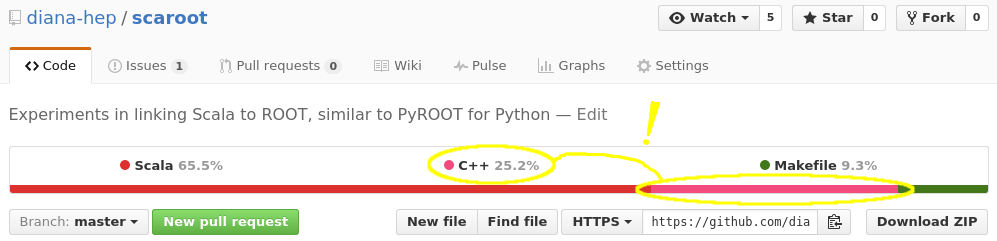
\includegraphics[width=\linewidth]{scaroot_languages.png}

\vspace{0.2 cm}
\begin{itemize}
\item Tested JNI (unsuccessfully) and JNA (successfully).
\begin{itemize}
\item Can open ROOT file and print {\tt ->ls()} from Scala.
\end{itemize}
\item Set up a clean build environment with Maven and Make:
\begin{itemize}
\item {\tt mvn install} command runs {\tt make} to build C++ first, then Scala (mixed with any Java, if needed).
\item C-style symbol names ({\tt extern "C"}) in {\tt scaroot.so}.
\item {\tt scaroot.so} enclosed within {\tt scaroot.jar}.
\item User submits only {\tt scaroot.jar} to the Spark cluster, but {\tt LD\_LIBRARY\_PATH} must be pointing to ROOT on the cluster.
\item Perhaps I can encapsulate a whole version of ROOT in the {\tt scaroot.jar}, so the whole thing gets sent with the workflow.
\end{itemize}
\item Namespace: {\tt org.dianahep}, GroupID: {\tt org.diana-hep}.
\end{itemize}
\end{frame}

\begin{frame}[fragile]{src/main/cpp/scaroot.cpp}
\begin{lstlisting}[language=c++]
#include <stdint.h>
#include "TFile.h"

extern "C" {
  int64_t new_TFile(char *fileName);
  void delete_TFile(int64_t pointer);
  void TFile_ls(int64_t pointer);
}

int64_t new_TFile(char *fileName) {
  TFile *tfile = new TFile(fileName);
  return (int64_t)tfile;
}

void delete_TFile(int64_t pointer) {
  TFile *tfile = (TFile*)pointer;
  delete tfile;
}

void TFile_ls(int64_t pointer) {
  TFile *tfile = (TFile*)pointer;
  tfile->ls();
}
\end{lstlisting}
\end{frame}

\begin{frame}[fragile]{src/main/scala/org/dianahep/scaroot/Main.scala}
\begin{lstlisting}[language=java]
package org.dianahep

import com.sun.jna._

package scaroot {
  object SharedObject extends Library {
    Native.register("/resources/native/scaroot.so")
    @native def new_TFile(fileName: String): Long
    @native def delete_TFile(pointer: Long): Unit
    @native def TFile_ls(pointer: Long): Unit
  }

  object Main {
    def main(args: Array[String]) {
      val pointer = SharedObject.new_TFile("Event.root")
      println(s"pointer value $pointer")
      SharedObject.TFile_ls(pointer)
      println(s"see a listing?")
      SharedObject.delete_TFile(pointer)
      println(s"still here?")
    }
  }
}
\end{lstlisting}
\end{frame}

\begin{frame}[fragile]{src/main/cpp/Makefile}
\small
\begin{lstlisting}[language=sh]
all: scaroot.cpp
    g++ -fPIC -shared -Wl,--no-as-needed \
        $(shell root-config --cflags --ldflags --libs) \
        -o ../../../src/main/resources/native/scaroot.so \
        scaroot.cpp
\end{lstlisting}

\vfill
\hspace{-0.83 cm} \textcolor{darkblue}{\Large {\tt pom.xml} fragment}
\begin{lstlisting}[language=XML]
...
<plugin>
  <groupId>org.codehaus.mojo</groupId>
  <artifactId>exec-maven-plugin</artifactId>
  <executions>
    <execution>
      <phase>generate-sources</phase>
      <goals><goal>exec</goal></goals>
      <configuration>
        <workingDirectory>src/main/cpp</workingDirectory>
        <executable>make</executable>
      </configuration>
...
\end{lstlisting}
\end{frame}

\begin{frame}[fragile]{Directory structure}
\small
\dirtree{%
.1 scaroot.
.2 pom.xml.
.2 README.md.
.2 src.
.4 main.
.5 cpp.
.6 Makefile.
.6 scaroot.cpp.
.5 resources.
.6 native.
.5 scala.
.6 org.
.7 dianahep.
.8 scaroot.
.9 Main.scala.
.4 test.
.5 scala.
.6 test.scala.
}
\end{frame}

\end{document}
